\documentclass{article}
\usepackage{hyperref}
\usepackage[utf8]{inputenc}
\usepackage[english]{babel}
\usepackage{amsmath}
\usepackage{todonotes}
\usepackage{siunitx}
\usepackage{float}
\usepackage{booktabs}
\usepackage{listings}
\sisetup{locale=DE}

\definecolor{mygreen}{RGB}{28,172,0}
\definecolor{mylilas}{RGB}{170,55,241}

\newcommand{\norm}[1]{\left\lVert#1\right\rVert}

\lstset{language=Matlab,%
    %basicstyle=\color{red},
    breaklines=true,%
    morekeywords={matlab2tikz},
    keywordstyle=\color{blue},%
    morekeywords=[2]{1}, keywordstyle=[2]{\color{black}},
    identifierstyle=\color{black},%
    stringstyle=\color{mylilas},
    commentstyle=\color{mygreen},%
    showstringspaces=false,%without this there will be a symbol in the places where there is a space
    numbers=left,%
    numberstyle={\tiny \color{black}},% size of the numbers
    numbersep=9pt, % this defines how far the numbers are from the text
    emph=[1]{for,end,break},emphstyle=[1]\color{red}, %some words to emphasise
}

\title{Computer Vision I - Sheet 3\\Group 2\\}
\author{ Jonas Otto\\ \href{mailto:jonas@jonasotto.com}{jonas@jonasotto.com} \and Dominik Authaler \\ 
\href{mailto:dominik.authaler@uni-ulm.de}{dominik.authaler@uni-ulm.de}
}

\date{\today}

\begin{document}
\maketitle

\newpage

\section{Histogram equalization}
The source code used for this task can be found beneath or in the file sh03ex01.m. Figure \ref{ex01} shows the results of this exercise. The left part of the figure shows the original image together with it's histogram and the cumulative histogram. The right part shows the improved image, which was received after applying an equalization to the histogram. Therefore the cumulative histogram now shows some linear behaviour. As can be seen in the code we used a lookup-table for mapping between the original intensity value and the new intensity value.

\hspace{20mm}
\lstinputlisting{./matlab/sh03ex01.m}

\begin{figure}[H]
  \begin{center}
    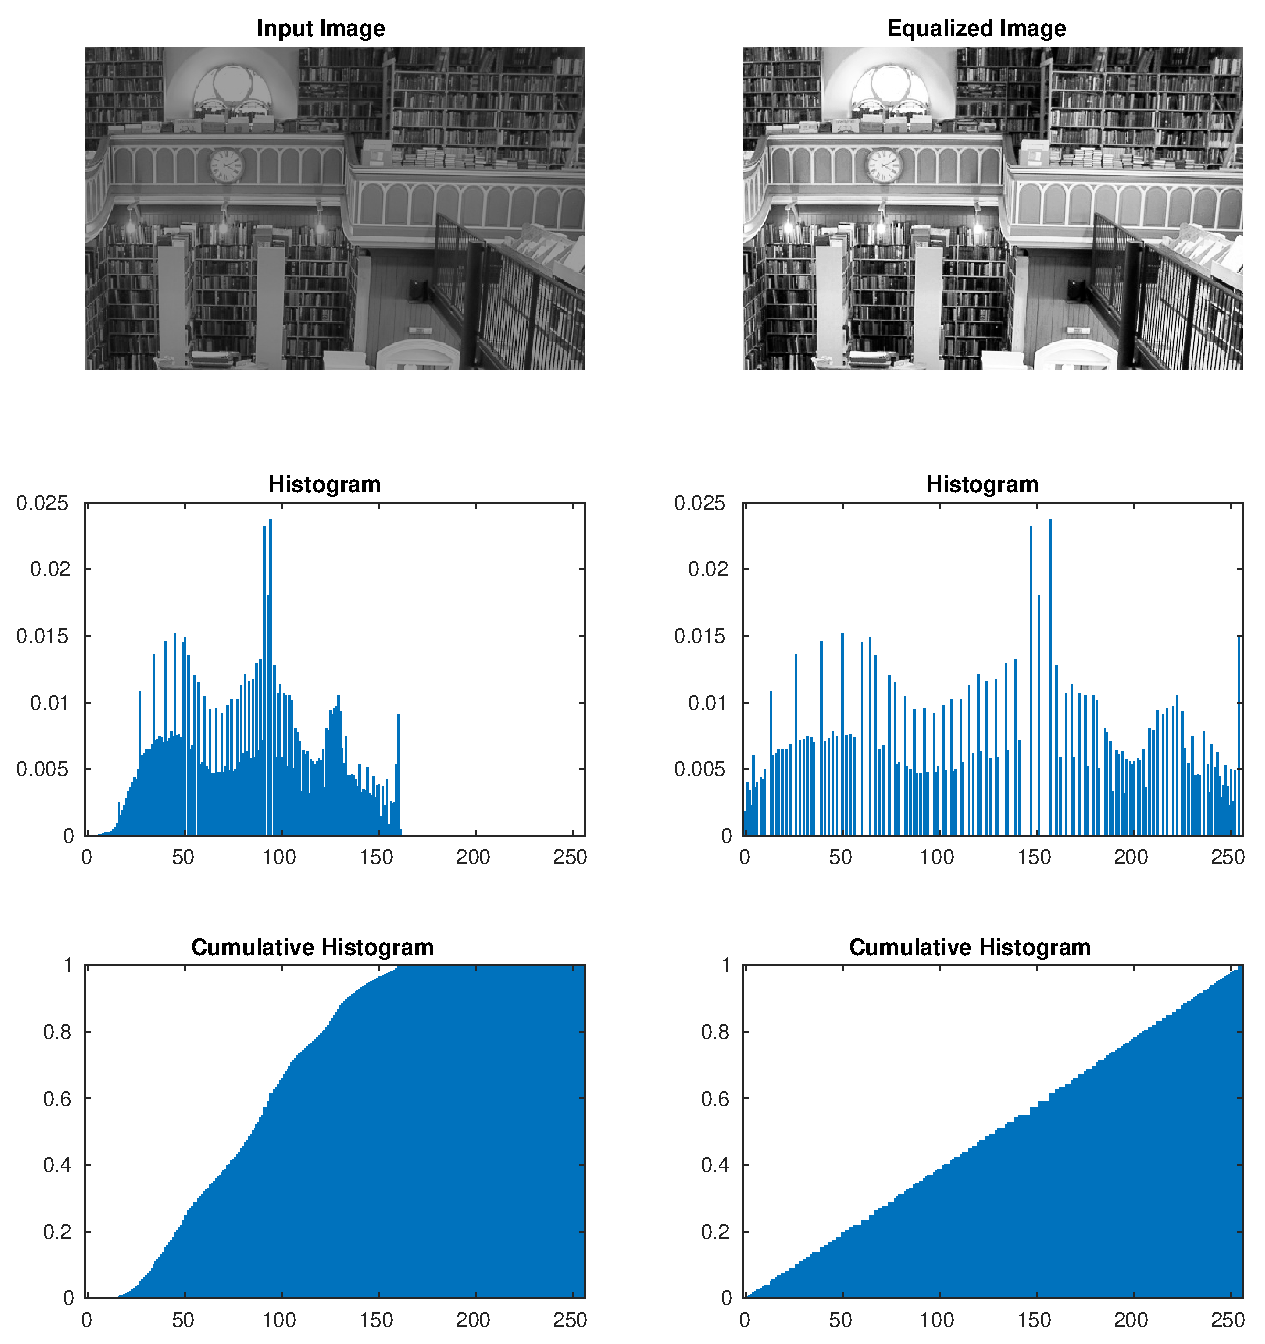
\includegraphics[width=\textwidth]{./images/ex01.eps}
    \caption{Results of exercise 1}
    \label{ex01}
  \end{center}
\end{figure}

\clearpage
\section{Image gradients}
The sign of the sobel operator decides whether the result approximates the gradient or the negative gradient. The resulting vector points towards the biggest increase if the sign is positive, therefore if one inverts the sign of both Sobel operators it would point to the biggest decrease. Nevertheless, the length of the gradient vector stays the same.

For the second task one needed to be aware that the y-axis points downwards, although the thoughts behind Sobel operators assumed a "normal" mathematical coordinate system. Therefore we either need to multiply the Sobel operator for the y-direction with $-1$ or the result $I_y$ calculated with the given kernel. We've chosen the latter approach. The results for the different positions given in task 2 can be found in Table \ref{tab1}. For the positions $v_2$ and $v_4$ there is no nice rational fraction times $\pi$. Therefore this results are approximately given as a decimal number in radians.

\begin{table}[H]
  \centering
  \label{tab1}
  \caption{Results of exercise 2.2}
  \begin{tabular}{cccc}
    \toprule
    Position $v_i$ & $(I_x, I_y)$   & $\norm{\nabla I(v_i)}$ & $\theta_i$        \\
    \midrule
    $v_1$          & $(-255, 255)$  & $360.624$              & $\frac{3}{4}\pi$  \\
    $v_2$          & $(765, 255)$   & $806.381$              & $0.322$           \\
    $v_3$          & $(-255, -255)$ & $360.624$              & $-\frac{3}{4}\pi$ \\
    $v_4$          & $(-255, -765)$ & $806.381$              & $-1.892$          \\
    $v_5$          & $(-1020, 0)$   & $1020$                 & $-\pi$            \\
    $v_6$          & $(765, -765)$  & $1081.873$             & $-\frac{1}{4}\pi$ \\
    \bottomrule
  \end{tabular}
\end{table}

The source code used to generate the images shown in figure \ref{ex02} can be also found in the file sh03ex02.m. For the visualization of the original image we let Matlab rearrange the intensity values over the full range from 0 to 255, therefore the circles look brighter/darker than one would expect from their original intensity values.

\hspace{20mm}
\lstinputlisting{./matlab/sh03ex02.m}


\begin{figure}[H]
  \begin{center}
    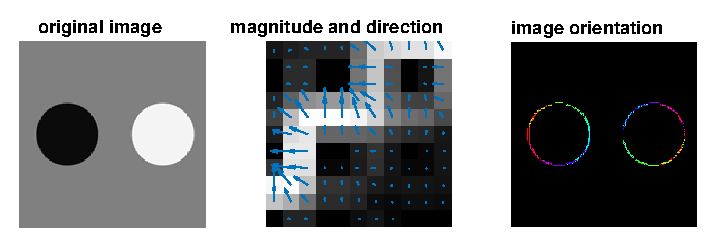
\includegraphics[width=\textwidth]{./images/ex02.eps}
    \caption{Results of exercise 2}
    \label{ex02}
  \end{center}
\end{figure}

\clearpage
\section{Deconvolution}
The source code seen below can also be found in file sh03ex03.m. Figure \ref{ex03_filters} shows the given filters both in the spatial and the frequency domain. Because most of the image in the spatial domain is filled with zero, this plot only shows the range from 1 to 30 in y-direction and 1 to 50 in x-direction. Figure \ref{ex03_images} displays the original image together with the blurred image and the two images gained from the deconvolution operation applied on the blurred image for both filters.
Comparing the original image with the resulting one of the deconvolution operation with filter 1, there aren't any obvious differences, whereas the difference to second deconvolved image is huge. Thus it seems like the filtered image was constructed using the first filter in a convolution operation.

Important for the abitity to reconstruct an image completely is, that the filter mustn't contain any zero values in the frequency domain, because these values can't be changed any more by the deconvolution operation.


\hspace{20mm}
\lstinputlisting{./matlab/sh03ex03.m}

\begin{figure}[H]
  \begin{center}
    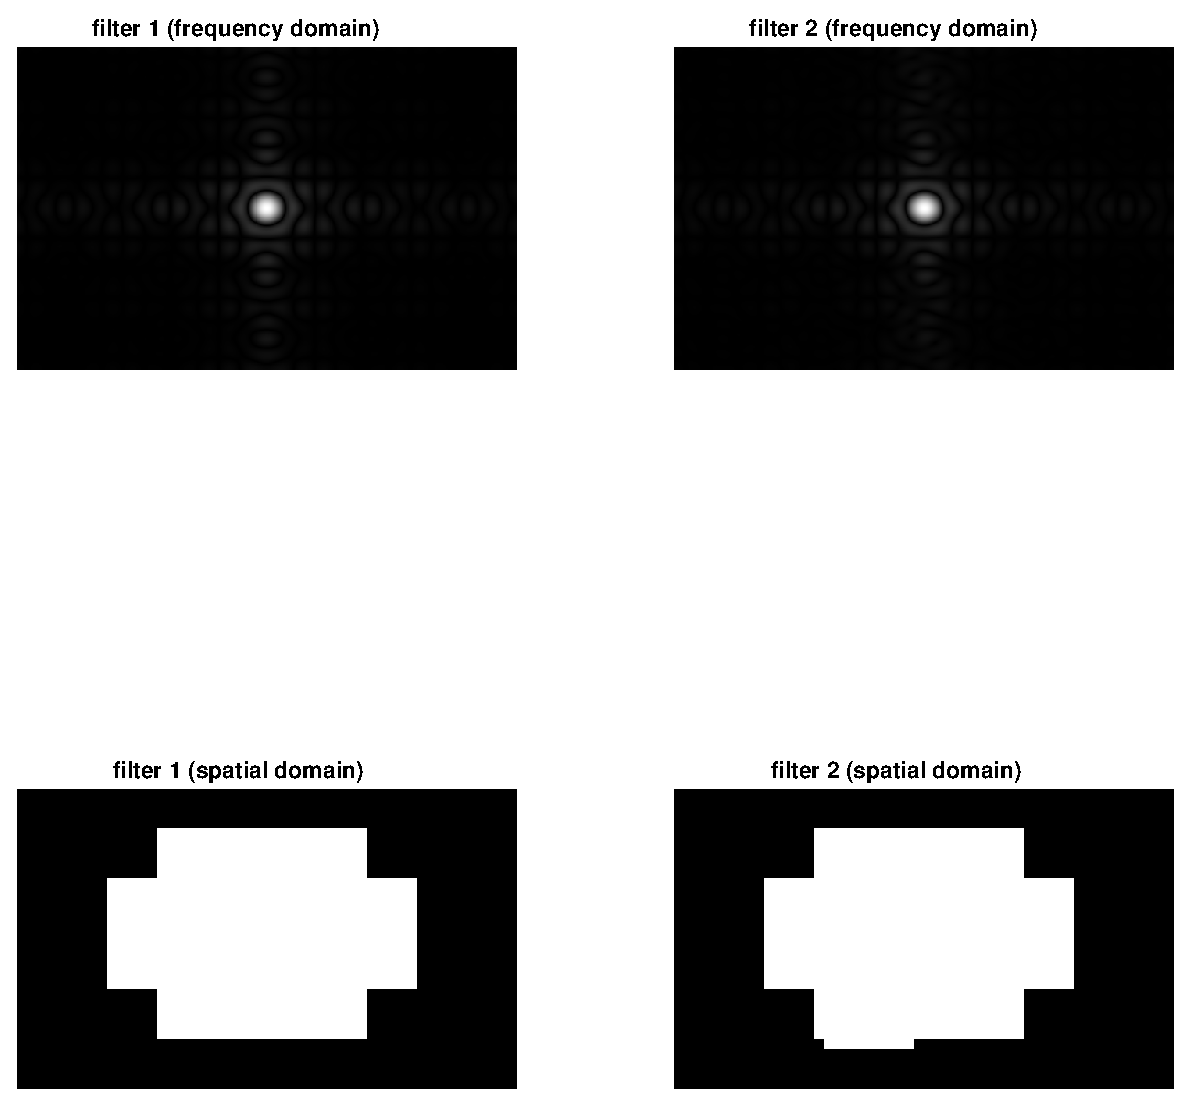
\includegraphics[width=\textwidth]{./images/ex03_filters.eps}
    \caption{Filters used in exercise 3}
    \label{ex03_filters}
  \end{center}
\end{figure}

\begin{figure}[H]
  \begin{center}
    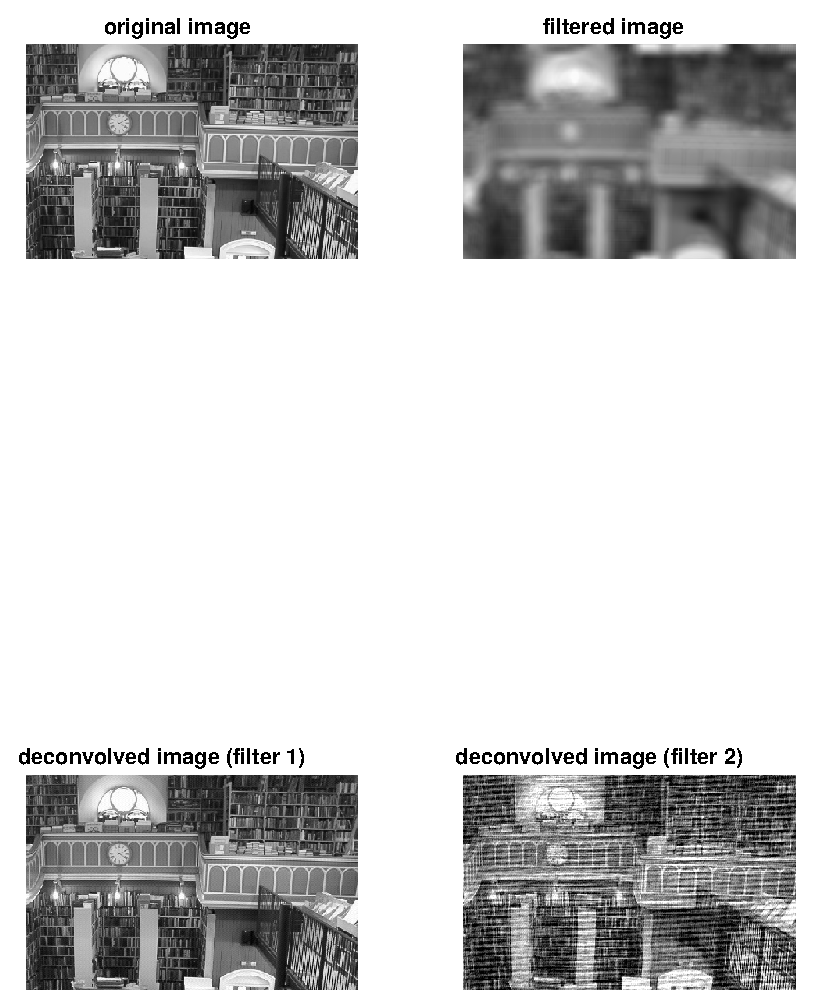
\includegraphics[width=\textwidth]{./images/ex03_images.eps}
    \caption{Resulting images in exercise 2}
    \label{ex03_images}
  \end{center}
\end{figure}

\end{document}

